
\documentclass[11pt, titlepage]{article}
\usepackage{psdiproject_report}

%%%%%%%%%%%%%%
%Instructions%
%%%%%%%%%%%%%%
%Edit the section below replacing the capitalised text with the information for the specific report
%Complete the sections of the report as necessary
%%%%%%%%%%%%%%

%%%%%% EDIT THIS SECTION %%%%%%
%replace the capitalised text with the relevant information - don't remove the \xspace
\newcommand{\teamnumber}{3\xspace}  %INSERT TEAM NUMBER HERE
\newcommand{\projectname}{Machine Learning Models to Predict Miscibility\xspace} %INSERT PROJECT NAME HERE
\newcommand{\studentlist}{Daniel Nathan Tomas Cancado, Thasmia Fathima Mohamed Aleem Basha, Joshua Cheung\xspace}  %INSERT TEAM LIST HERE
\newcommand{\reportdate}{24 July 2023\xspace} %INSERT PUBLISHED DATE HERE dd/mm/yyyy
\newcommand{\reporttitle}{PSDI-Intern-Series-2023:Report[3]\xspace} %replace x with report number - S.Kanza will provide this
\newcommand{\doi}{DOI HERE} %INSERT DOI HERE - S.Kanza will provide this

%%%%%%
% Can also use the following commands for AI4SD names
% \AISDLong gives - AI 4 Science Discovery Network+
% \AISDShort gives - AI4SD

%%%%%
%Inserting graphics %
%\begin{figure}[h]
%\centering
%\includegraphics[width=\textwidth]{./media/filename}
%\caption{caption }
%\end{figure}
\setlength{\parindent}{0pt}
\hypersetup{citecolor=blue}
\begin{document}

\PSDITitlePage{}
\publishinginfo{}
\PSDIContents{}

\setcounter{page}{1}
\section{Project Details}

\begin{table}[H]
\centering
\begin{tabular}{|p{1.5in}|p{4.5in}|}
\hline
Team Number & {\teamnumber} \\
\hline
Project Name & {\projectname} \\
\hline
Project Dates & 12th June - 24st July \\
\hline
Website & 
\href{xxx}{https://github.com/joooshc/PSDI-Miscibility} \\
\hline
\end{tabular}
 \end{table}

\section{Project Team}
\subsection{Project Student}
\begin{table}[H]
    \centering
    \begin{tabular}{|p{2in}|p{4in}|}
        \hline
        \textbf{Name and Title} & Daniel Nathan Tomas Cancado \\
        \hline
        \textbf{University Department Name} & 
        Electronics and Computer Science \\
        \hline
        \textbf{Work Email} & 
        dc1n19@soton.ac.uk \\
        \hline
        \textbf{Website Link (if available)} & 
        N/A \\
        \hline      
    \end{tabular}
\end{table}

\begin{table}[H]
    \centering
    \begin{tabular}{|p{2in}|p{4in}|}
        \hline
        \textbf{Name and Title} & Thasmia Fathima Mohamed Aleem Basha \\
        \hline
        \textbf{University Department Name} & 
        Eng Ed - Mechanical Engineering \\
        \hline
        \textbf{Work Email} & 
        tmab1g21@soton.ac.uk \\
        \hline
        \textbf{Website Link (if available)} & 
        N/A \\
        \hline      
    \end{tabular}
\end{table}

\begin{table}[H]
    \centering
    \begin{tabular}{|p{2in}|p{4in}|}
        \hline
        \textbf{Name and Title} & Joshua Cheung \\
        \hline
        \textbf{University Department Name} & School of Chemistry \\
        \hline
        \textbf{Work Email} & jc10g22@soton.ac.uk \\
        \hline
        \textbf{Website Link (if available)} & N/A \\
        \hline      
    \end{tabular}
\end{table}

\subsection{Project Supervisor}

\begin{table}[H]
    \centering
    \begin{tabular}{|p{2in}|p{4in}|}
        \hline
        \textbf{Name and Title} & Dr. Jo Grundy \\
        \hline
        \textbf{University Department Name} & 
        Electronics and Computer Science \\
        \hline
        \textbf{Work Email} & 
        j.grundy@soton.ac.uk \\
        \hline
        \textbf{Website Link (if available)} & 
   \href{xxx}{https://www.southampton.ac.uk/people/5xrlgf/doctor-jo-grundy}\\
        \hline      
    \end{tabular}
\end{table}

\subsection{Project Description}
\label{section:challenge}
The foundation of any successful machine learning model lies in the quality of the training data. To obtain accurate predictions, it is crucial that the dataset has well-established labels for classification or values for regression. In this project, several models were trained to predict mole fractions based on true values taken from datasets supplied by The International Union of Pure and Applied Chemistry (IUPAC). \\

The concept of mole fraction represents the ratio of moles of one substance in a mixture to the total number of moles in all of the substances. This is linked to Raoult's Law, which describes the behaviour of two liquids forming a single-phase mixture. According to this law, the partial pressure of two liquids is related to the total vapour pressure, and depends on their respective mole fractions \cite{1991223}. In this way, mole fractions can represent a uniform mixture, considering that both liquids contribute equally to the final partial pressure. Therefore, Raoult's Law can potentially help to determine whether the interaction is fully or partially miscible. Since pressure is related to temperature in thermodynamics, it's possible to consider the effects of variations in temperature instead of pressure with respect to mole fractions. \\

IUPAC \cite{iupac} has solubility datasets (SDS), many of which contain a mixture of two liquids. As mole fractions and temperatures appear quite often in SDS volumes, it offers a chance to explore the relationship between them and their respective temperatures, as well as how they may indicate complete miscibility. The goal of this project is to train predictors for the mole fraction of two organic compounds at a set temperature, offering a suitable approach to predict miscibility using a model built on undigitised solubility datasets. \\

\section{Lay Summary}
\label{section:Lay Summary}
This project focused on using machine learning (ML) to predict how well different liquids mix together to form a uniform solution. The key to making accurate predictions was having a large and reliable dataset with information about how these substances mix. A property called mole fraction was used, which represents the proportion of each substance present in the mixture. By determining the mole fraction, it might be possible to say how well two liquids can mix at a given temperature.\\

Various ML models (Linear, Polynomial, Random Forest, Gradient Boosting, and Neural Networks) were trained and tested using IUPAC data, which included information about different mixtures and their mole fractions at specific temperatures. Ensemble learning methods, such as Random Forest and Gradient Boosting, showed promising results. These methods combine the knowledge of many individual models to make better predictions. For example, the random forest model works by taking the average of predictions from different models to form a final reliable prediction, and gradient boosting learns from the mistakes of previous models to improve its predictions. However, the most accurate model was a Feed Forward Neural Network, which processes input data through interconnected inputs, referred to as neurons, to learn patterns in the data necessary to make accurate predictions.\\ 

Several challenges were encountered due to limited data on miscibility and the need for manual data pre-processing. The models were tested within specific temperature ranges, potentially affecting their reliability for extrapolation to other temperatures. Nevertheless, the project demonstrated the potential of ML in predicting mole fractions of mixtures. Further research could address the models' limitations and enhance their applicability to a broader range of conditions and substances, opening up new possibilities for optimising mixtures in various industries.

\section{Introduction}
\label{section:introduction}
Miscibility is a property of liquids that governs their ability to combine to form a homogeneous mixture. Accurately predicting the miscibility of liquids is crucial in various sectors, with the pharmaceutical industry being one of the most important.\\

One such example is the case of Ritonavir, a medication used to treat HIV/AIDS \cite{ritonavir}. In 1998, supplies were threatened as a result of the formation of a significantly less soluble crystal form of Ritonavir.  Form II had a lesser bioavailability due to its less soluble nature, which decreased its effectiveness. \cite{ritonavir2} Ultimately, this issue resulted in a loss of \$250 million in revenue \cite{ritonavir3}
By using ML methods to predict the miscibility of solvents, drugs or the coating for drugs can be created with specific properties that enhance therapeutic efficiency.\\

Three distinct data processing methods were tested and fundamental scoring metrics including Mean Squared Error (MSE) and $R^{2}$ were used. To choose the best model, the accuracy of the output from a variety of models including Linear, Polynomial and Random Forest regression, Gradient Boosting, and Neural Networks were assessed. Despite attempts to create a robust strategy to predict miscibility using machine learning models, issues stemming from data scarcity were a prominent challenge. These limitations led to the research statement:\\\\
\textit{"Utilising machine learning models to predict the mole fraction of compounds at a specified temperature using limited labelled and unlabelled data."}

\section{Methodology}
\label{section:methodology}

\begin{figure}[ht]
\centering
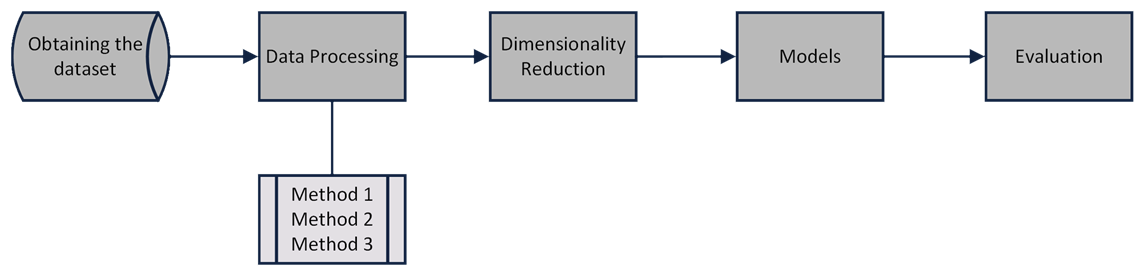
\includegraphics[width=15cm]{./media/methodology.png}
\caption{A flow diagram of the methodology process}
\end{figure}

\subsection{Obtaining the Dataset}
The primary challenge faced at the project's onset was the lack of usable data. The IUPAC solubility dataset, the largest dataset of solubility data, consists of approximately 100 different pdfs, many of which were written using a typewriter and then scanned and uploaded online. For machine learning, this raw data was unsuitable. Consequently, over 900 compound pairs were typed up along with their corresponding mole fractions and temperatures into a json file. The mole fraction provided the "y" for the model, and the temperature provided the first of the "X".\\

To expand the "X" for the model, i.e., the features, a variety of methods were tested: PubChemPy\cite{PubChem}\cite{PubChemPy} (Python PubChem API), CIRpy\cite{CIRpy} (Chemical Identifier Resolver Python API), and RDKit\cite{RDKit}. Some compounds didn't have data with one or more of the chosen methods, resulting in their exclusion and an overall data loss of roughly 10\% from the original collected data. For this reason, MACCs keys from RDKit were not used in the final dataset, as they caused too much data loss.

\subsection{Data Preprocessing}
The differences between the features of the two compounds were calculated (e.g., molecular mass 1 - molecular mass 2), and the Sci-Kit Learn\cite{sklearn} pre-processing module was used for scaling the features. This helped to ensure that some features weren't discarded due to having an unidentifiable distribution, a problem primarily caused by the small size of the dataset. Scaling also affects model performance, as seen in the results.\\

The scaling was evaluated visually using histograms. During the development phase, several different methods of scaling the dataset were used:
\subsubsection{Method 1}
In the first version of the scaled dataset, all the data was scaled using the StandardScaler function from Scikit-learn. Columns containing only 0 or 1 were removed, but the data was not processed in any other way. Unsurprisingly, this gave incredibly poor results in the model.

\begin{figure}[ht]
\centering
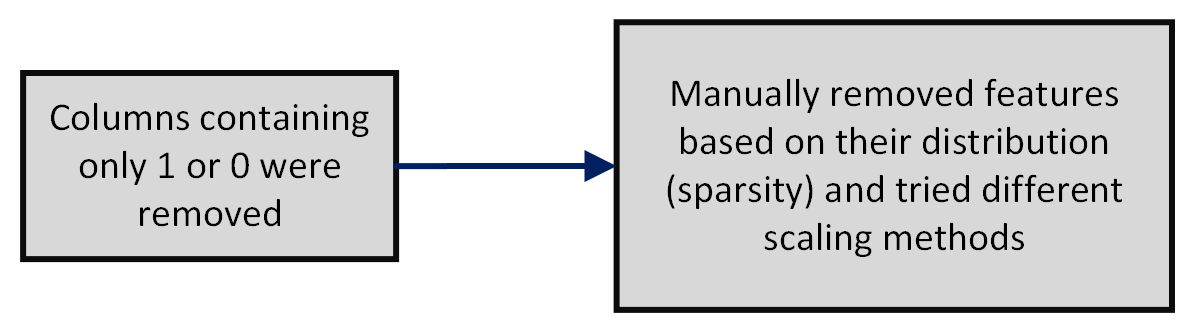
\includegraphics[width=8cm]{media/Method1.png}
\caption{A flow diagram of method 1 scaling}
\end{figure}

\subsubsection{Method 2}
When the histogram of the raw data was too sparse (1-3 bins filled), the feature was removed. The following functions were trialled: square root, log, quantile, min-max and standard. Outliers were removed if they fell greater than 3 standard deviations away from the mean. This worked with varying success.

\begin{figure}[ht]
\centering
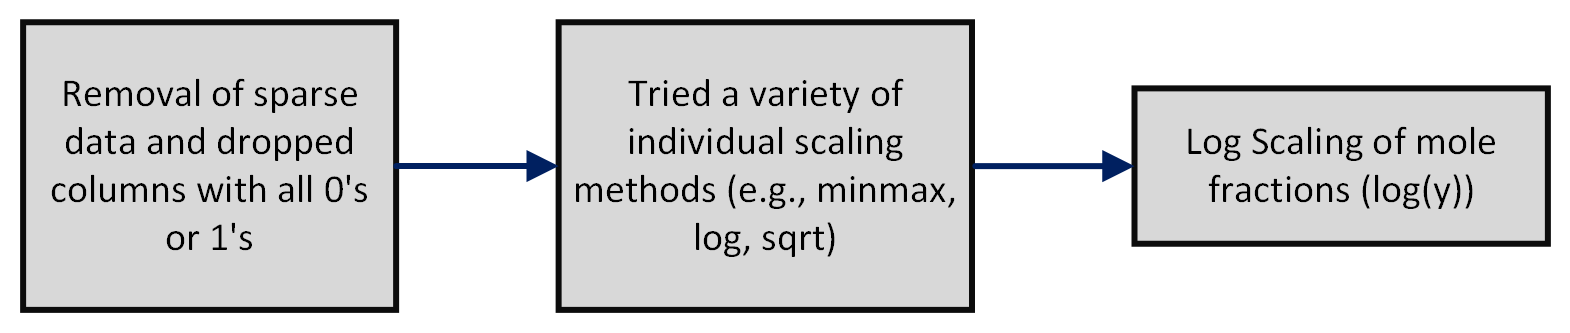
\includegraphics[width=12cm]{media/Method2.png}
\caption{A flow diagram of method 2 scaling}
\end{figure}

Method 2 (other):\\
This method was the same as the main method 2, but different scaling functions were chosen based on the distribution of the raw unprocessed data. The result of this scaling was mostly satisfactory, but several features still had a very skewed histogram.\\

\subsubsection{Method 3}
Initial processing was done in a similar way to method 2, with removal of features that contained sparse data. All the data was normalised, followed by quantile scaling to fit a normal distribution, then log scaling. This yielded acceptable results, but not the best.

\begin{figure}[ht]
\centering
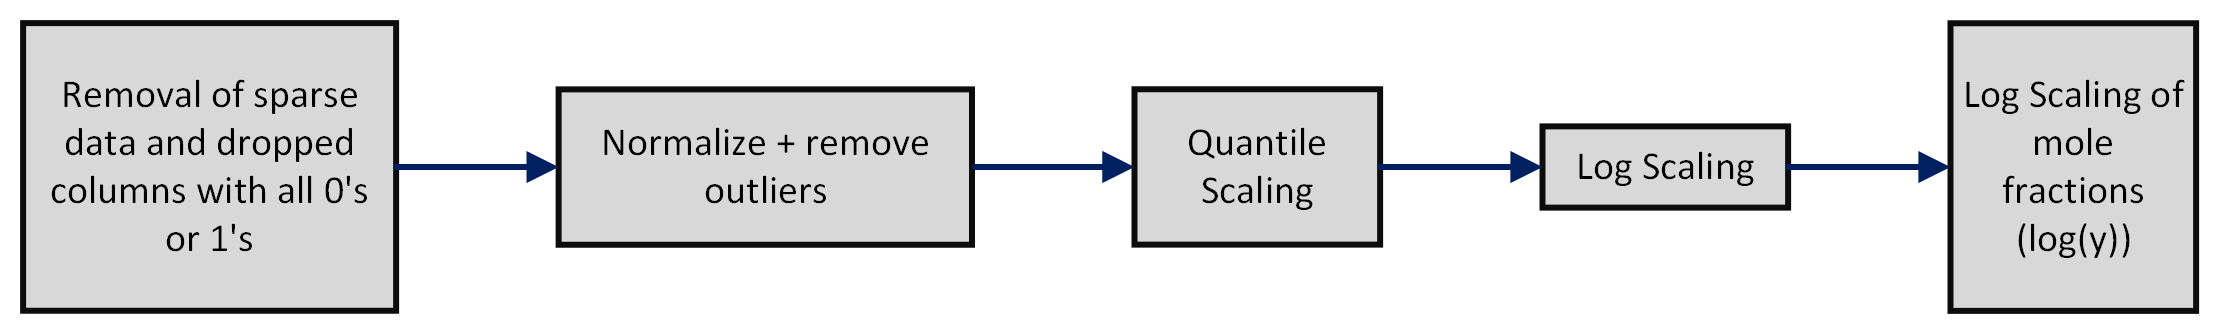
\includegraphics[width=12cm]{media/Method3.png}
\caption{A flow diagram of method 3 scaling}
\end{figure}

\begin{table}[h!]
\centering
\begin{tabular}{|c|c|}
\hline
\textbf{Scaling Method} & \textbf{Transformation} \\ 
\hline
Square Root & $y=\sqrt{x}$ for $x>0$, $y=\sqrt{x-x_\text{min} +1}$ for $x\leq0$ \\ 
\hline
Log & $y=\ln{x}$ for $x>0$, $y=\ln(x-x_\text{min}+1)$ for $x\leq0$ \\ 
\hline
Quantile & $x$ is ranked, then scaled with the ranking to a normal distribution. \\ 
\hline
Min Max & $x_\text{std} = \frac{x-x_\text{min}}{x_{max}-x_{min}}$, $y = x_\text{std}(1-0)+0$ \\ 
\hline
Standard & $y=\frac{x-\mu}{\sigma}$ \\ 
\hline
\end{tabular}
\caption{Transformation methods used for scaling features.}
\label{table:scaling}
\end{table}

\begin{figure}[ht]
\centering
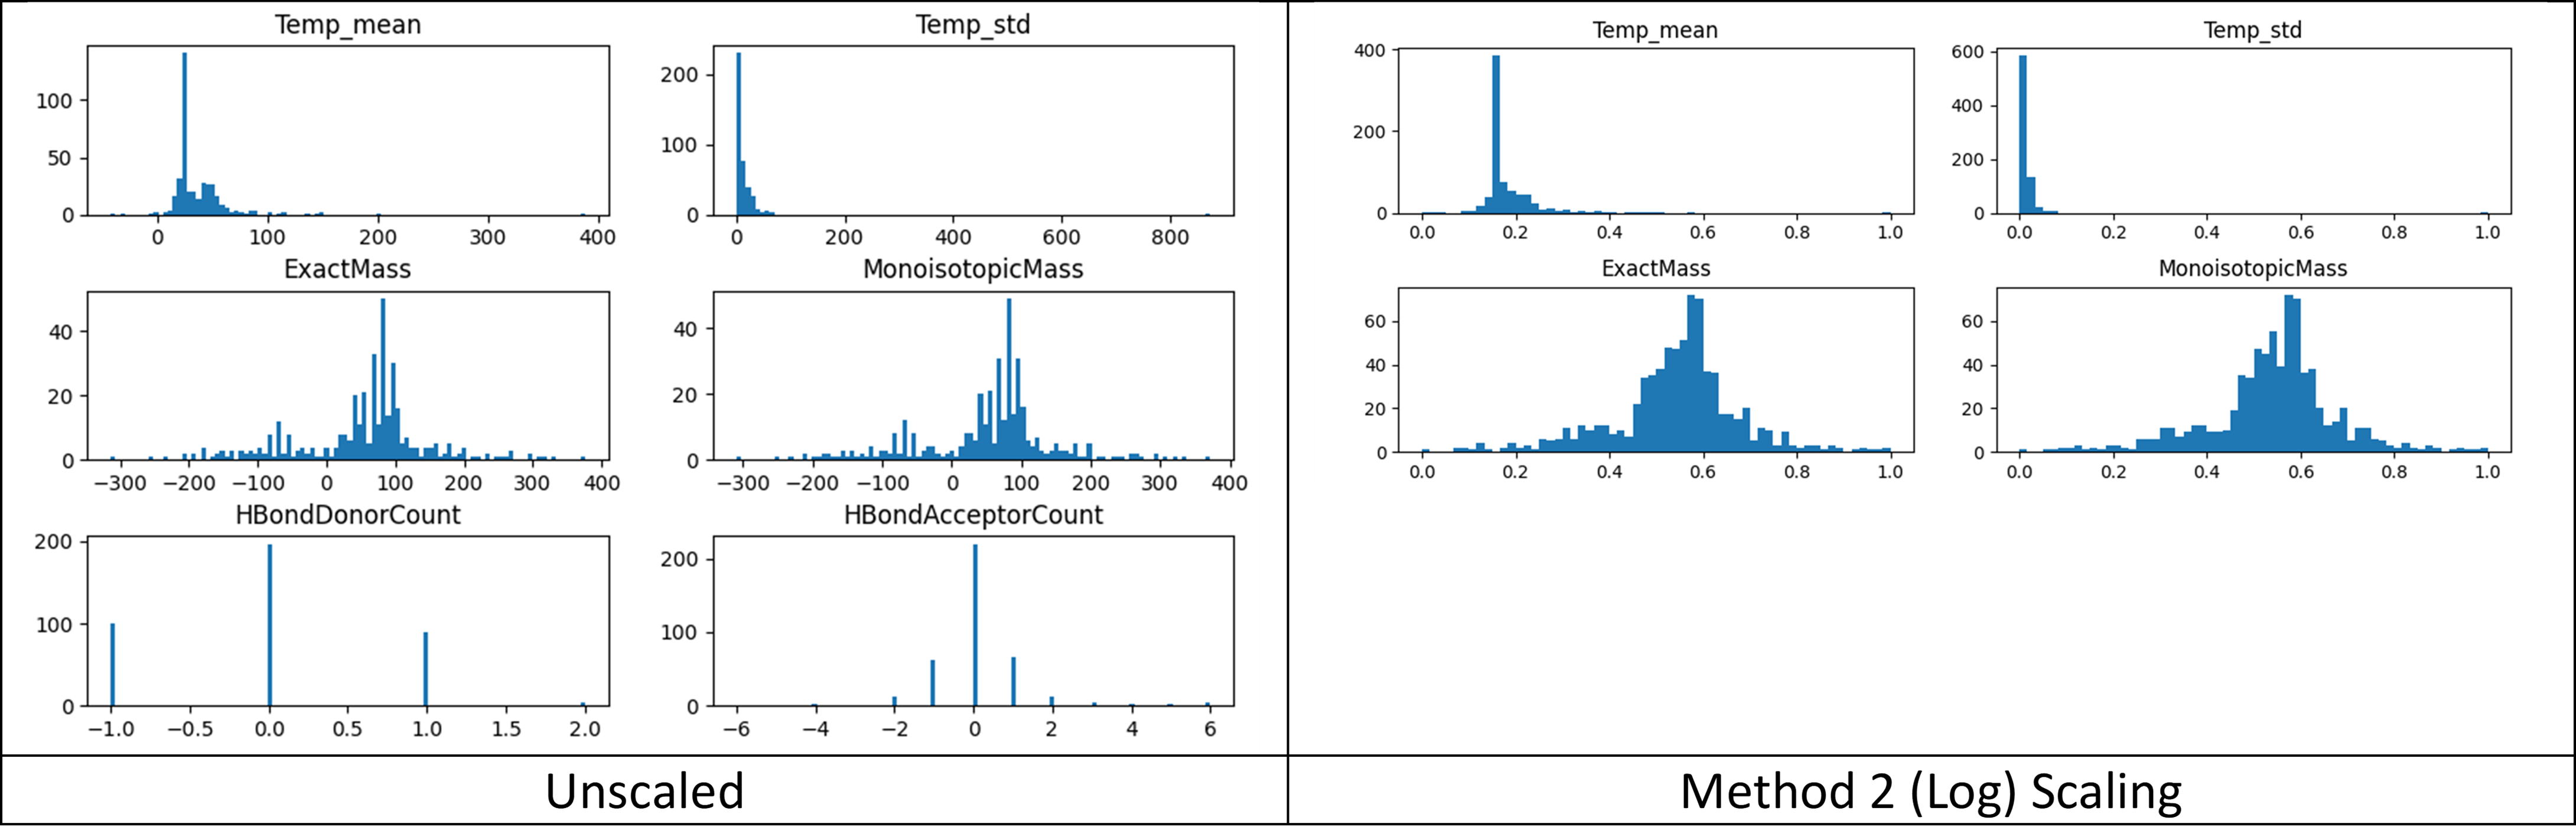
\includegraphics[width=16cm]{media/histograms.png}
\caption{Comparison of histograms before and after scaling}
\end{figure}
The side-by-side comparison of the histograms shows how the distribution of feature data is affected by the scaling methods used. It also shows the effect of removing outliers. A more even distribution of data is important for training the model because it ensures that the model is not skewed towards predicting the same thing every time. The figure also highlights the removal of features (e.g., HBondDonorCount and HBondAcceptorCount) that are sparse making it difficult to see any defined distribution - removing these improved our model's accuracy. 

\subsection{Dimensionality Reduction}
Principal Component Analysis (PCA) was used to reduce the dimensionality of the data. It finds and retains the most significant features of the data whilst minimising data loss. Using fewer PCA components helps to reduce the computational time and processing power required, but using too few components reduces the performance of the model overall. Using PCA components instead of features helps to avoid overfitting the data\cite{pca}.\\

To find the most suitable number of PCA components for each model, the models were tested with iterating numbers of components and the results were plotted. There was a positive correlation between the number of PCA components and the $R^{2}$ score until a certain limit for each model. This limit varied from model to model. For calculating the final evaluation metrics, each model was run on its "limit" of PCA components. This helped to strike the correct balance between producing optimum results for the model and saving processing power/computational time.

\subsection{Cross Validation}
Prior to training, our dataset was randomly sampled and split into smaller subsets, which were then used to validate training data for separate models. This method is known as Monte Carlo cross-validation \cite{montecarlo}. Randomly sampling test data is different to stratified k-fold cross-validation because although the training dataset is sampled and split into smaller test sets, with k-fold each are made up of unique samples \cite{kfold}. For example, where 20\% of the training set can be sampled 'n' times with Monte Carlo cross-validation, with k-fold, 'n' would be limited to five, seen as 20\% is one-fifth of the dataset - so as to ensure that each part holds distinct samples. \\

Monte Carlo cross-validation was used during training whereas k-fold was not. Ideally, it could have been used for our initial binary classification model (see report section 7). 

\subsection{The Models}
Multiple models were trialled in order to find the model that had the most accurate predictions for the data. Each model was tested and scored 10 times with randomly seeded 4:1 train test splits, and the average/standard deviation of its scores were used in evaluating them. Where applicable, a grid search was used to find optimum parameters for the model to achieve the best scores.

\subsubsection{Model Evaluation}
Models were scored by calculating the Mean Squared Error (MSE) and $R^2$ score. The mean, maximum, minimum, and standard deviation of these metrics were recorded each time.\\
\newline
Mean Squared Error:\\
$$\text{MSE} = \frac{\Sigma(y_{i}-\hat{y}_{i})^{2}}{n}$$
Mean squared error is a metric of the distance between the predicted y value and the true y value. The greater the error, the further the distance and the more inaccurate the model is\cite{mse}.\\
\newline
$R^{2}$ Score (Coefficient of Determination):\\
$$R^{2} = 1 - \frac{\Sigma_{i}(y_{i} - \hat{y_{i}})^{2}}{\Sigma_{i}(y_{i}-\bar{y})^{2}}$$
The $R^{2}$ score measures how well the predicted y values and the true y values correlate to each other\cite{r2}. A perfect correlation would have an $R^{2}$ value of 1. Normally, it falls between 0 and 1. However, when used as a metric on non-linear models, it can be negative, as discovered in model testing.

\subsubsection{Partial Least Squares Regression (PLS)}
PLS is a multivariate method that is often used when the number of features is greater than the number of datapoints\cite{pls1}. As a result, it is a useful alternative to try when OLS fails to produce good results. It is essentially an extension of multiple linear regression\cite{pls2}. It is implemented in Sci-Kit learn with the NonLinear Iterative Partial Least Squares (NIPALS) algorithm, created by Herman Wold, 1966\cite{nipals}.

\begin{table}[h!]
\centering
\begin{tabular}{|c|c|}
\hline
\textbf{Regression Model} & \textbf{Error Component ($\epsilon_{i}$)} \\ 
\hline
Ordinary Least Squares (OLS)\cite{ols} & $\Sigma_{i}\epsilon^{2}_{i} = \Sigma_{i}(y_{i}-\hat{y_{i}})^{2}$ \\ 
\hline
Lasso (L1)\cite{lasso} & $\Sigma_{i=1}^{n}(y_{i}-\Sigma_{j=1}^{p}X_{ij}\beta_{j})^{2}+\lambda\Sigma^{p}_{j=1}\vert\beta_{j}\vert$ \\ 
\hline
Ridge (L2)\cite{elastic} & $\Sigma_{i=1}^{n}(y_{i}-\Sigma_{j=1}^{p}x_{ij}\beta_{j})^{2}+\lambda\Sigma_{j=1}^{p}\beta_{j}^{2}$ \\ 
\hline
Elastic Net & $\Sigma_{i=1}^{n}(y_{i}-\beta_{0}-x^{T}_{i}\beta)^{2}+\lambda\Sigma^{p}_{j=1}(\beta^{2}_{j}+\alpha\vert\beta_{j}\vert)$ \\ 
\hline
\end{tabular}
\caption{Error component computation in various regression models.}
\label{table:regression_models}
\end{table}

\subsubsection{Linear Regression}
Linear regression works by modelling the relationship between two variables as a straight line by using a line of best fit.
$$y_{i} = \alpha + \beta x_{i} + \epsilon_{i}$$
where $\epsilon_{i}$ is the error component. When plotting the line of best fit, the model aims to minimise the error component as much as possible. Multiple variations of the linear regression model were used, each with a different way of calculating the error component.

\subsubsection{Polynomial Regression}
Polynomial regression is effectively just a case of linear regression\cite{poly} where instead of finding the relationship between X and y directly, the relationship between the polynomial features of X, and y is found - the design matrix of the data is analysed. As such, the polynomial regression model was tested with different loss functions: OLS, L1, L2 and elastic net were used.

\subsubsection{Random Forest Regression}
Random Forest is an ensemble learning method that uses a collection of decision trees to come up with a final robust prediction. Decision trees function by asking a true or false question, such as whether a given feature (e.g., temperature) fits within a certain threshold of variance. Depending on the answer, a node is split into two branches: one where the threshold of variance is met, and one where it is not \cite{randomforest}. The variance threshold is then refined further for subsequent nodes until a tree-like structure is complete. Random forest uses many of these trees (an ensemble) and takes the average of their final prediction.

\subsubsection{Gradient Boosting}
Two different boosting regressions were trialled: CatBoost and Gradient Boosting. Gradient Boosting is a method which combines the results of multiple models that progressively learn from one another in order to increase accuracy\cite{gradboost}. It starts with training a weak model (a linear regressor or decision tree for example), computes the residuals (errors between true vs predicted outputs) then trains subsequent models to make predictions for these residuals. Summing or subtracting residual predictions minimizes the error for the original predictions and with several iterations, the model can be fined tuned for an optimal output - a close as possible match to the target value. \\

A particular variant of Gradient Boosting is Categorical Boosting (CatBoosting). It specifically uses decision trees as the 'weak' model, and what makes it distinct from original Gradient Boosting is that it considers there to be an ordered relationship between features. This is likely to be the case seen as compound descriptors and properties are being used as inputs for their associated compound pairs, thus it would be reasonable to consider some kind of interdependency. CatBoost is an open-source boosting library developed by Yandex\cite{catboost}. 

\subsubsection{Neural Networks}
Deep Learning, although usually applied to classification problems, can also be useful for predicting continuous values such as mole fractions. While regression is often considered the default for such tasks, it's important to note that Artificial Neural Networks can be equally effective, or potentially superior. On this basis, we used a Feed Forward Neural Network for our analysis. \cite{DNN1} \\

A Feed Forward Neural Network allows data to flow in one direction. In every epoch, the input parameters (in this context, compound features) undergo weight adjustments within 'n' hidden layers. Then, an activation function is applied to the sum of these inputs, constraining them to a desirable range. The ReLU function was used to introduce non-linearity and efficiency in the network, and help mitigate the problem of vanishing gradients \cite{DNN2}. After minimizing the residuals to an acceptable level—determined by the learning rate and number of epochs, the processed values are then fed into an output layer consisting of a single neuron to produce a single output \\

During the data pre-processing stage, it was discovered that logarithmic scaling of outputs resulted in higher $R^2$ values. Thus, ensuring that the Neural Network could output negative in addition to continuous values was important. This was achieved by using a linear activation function on the output layer.
\newpage
\section{Results}
\label{section:results}
\subsection{Evaluation}
\begin{figure}[ht]
\centering
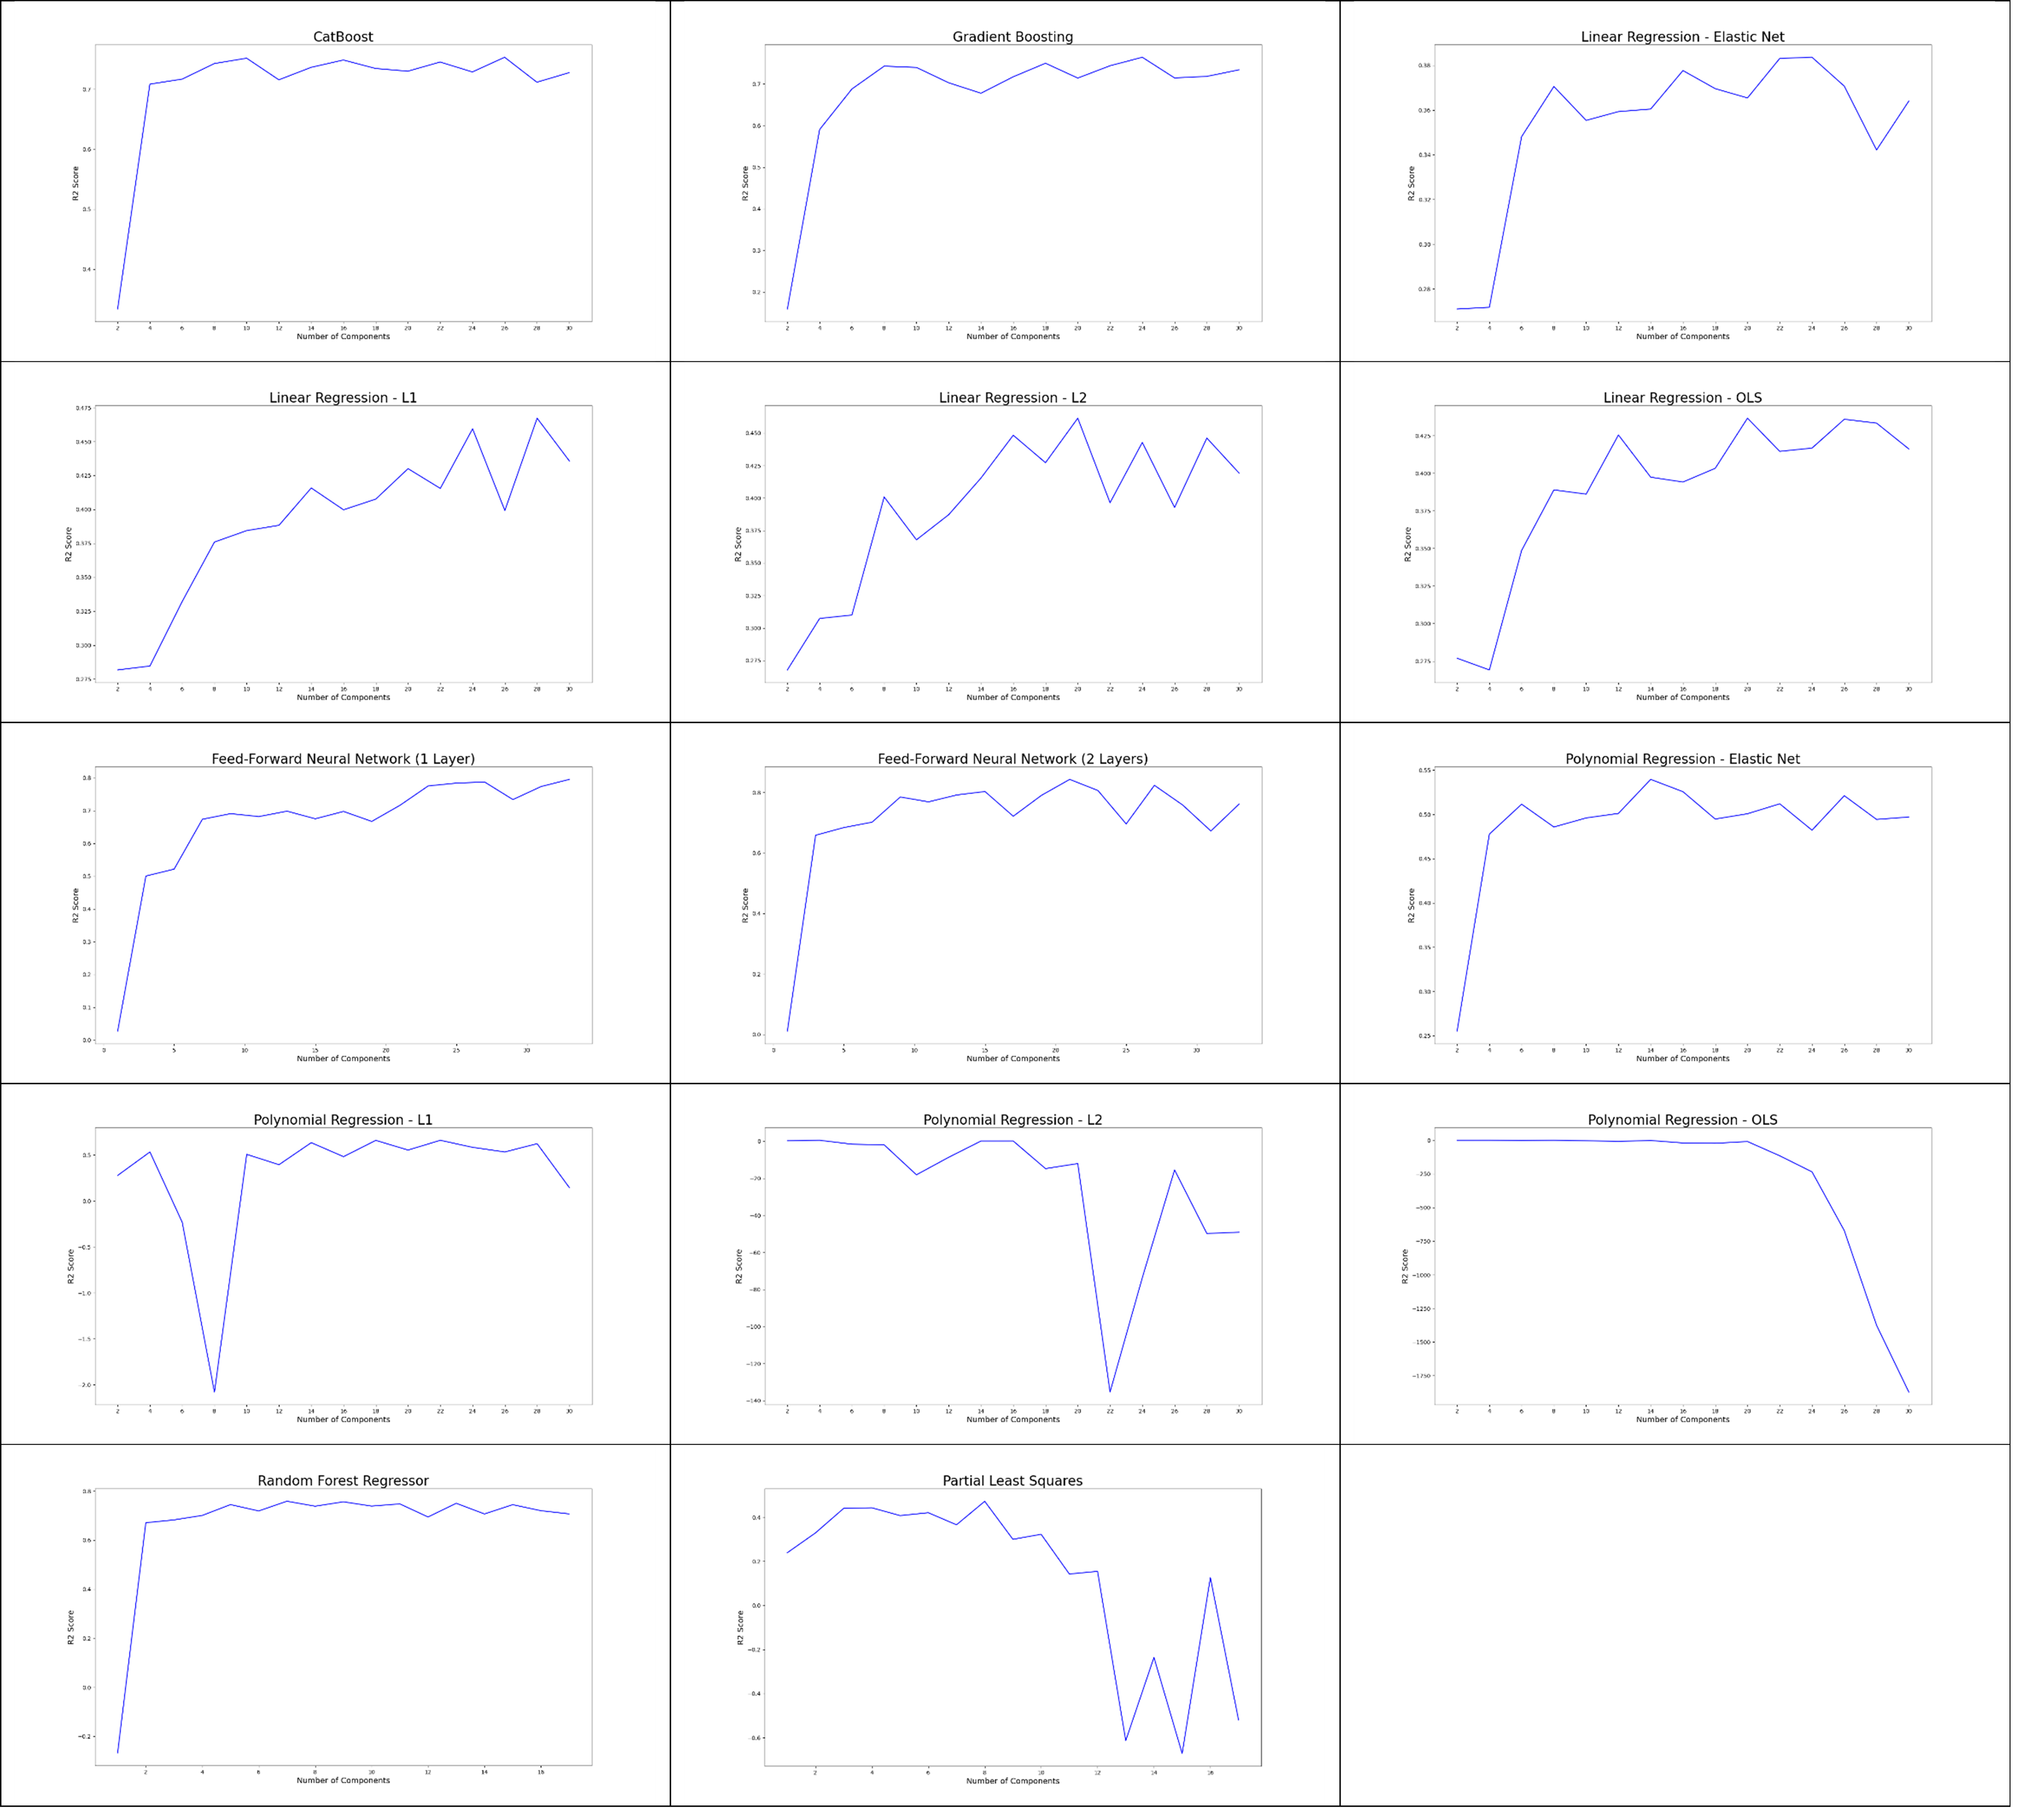
\includegraphics[width=16cm]{media/PCAiteration.png}
\caption{$R^{2}$ scores iterating across PCA components}
\end{figure} 

There was no clear relationship between the optimum number of PCA components for each model, but each model tended to perform best within a restricted range of components. Too many components increased the training time for the model, as well as the risk of overfitting the data.\\

As can be seen in Fig. 6, there were also cases where trained models with greater numbers of PCA components resulted in greater variation of $R^2$ scores (e.g., Partial Least Squares at PCA $>$ 20). This highlights the contrast between machine learning algorithms despite all being trained on the same datasets. The majority of the models tested have an exponential increase in $R^{2}$ score and asymptotically trend towards a maximum score. In contrast, polynomial regression with OLS has a similar but opposite effect, with an optimum with fewer components, and an exponential decay towards negative scores.\\

\begin{figure}[ht]
\centering
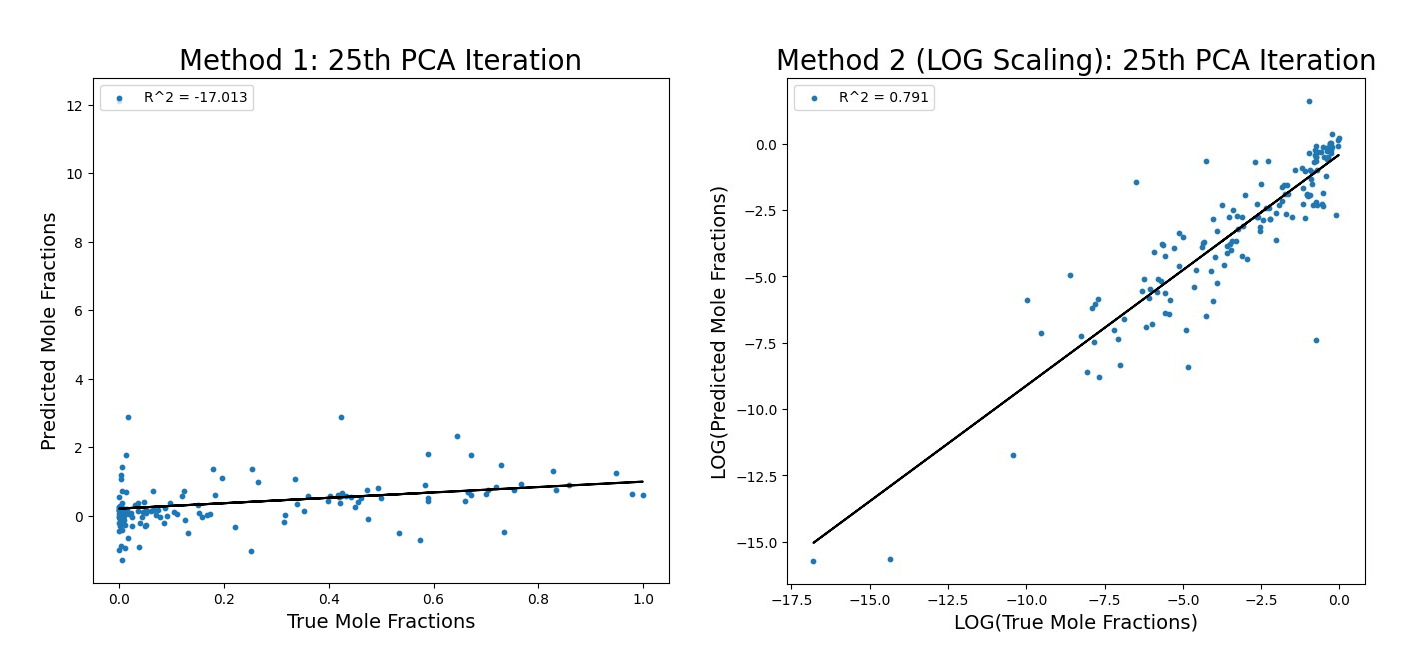
\includegraphics[width=16cm]{media/Scatters.png}
\caption{Results scatter plots for Neural Network (2 layers) model}
\end{figure}

\newpage

To highlight the difference between scaling methods, Fig. 7 shows two scatter plots and their respective scores. Simply applying the log transformation of targets and parameters had a massive effect on results; a positive correlation between true and predicted mole fractions was clearly visible.\\

\begin{figure}[ht]
\centering
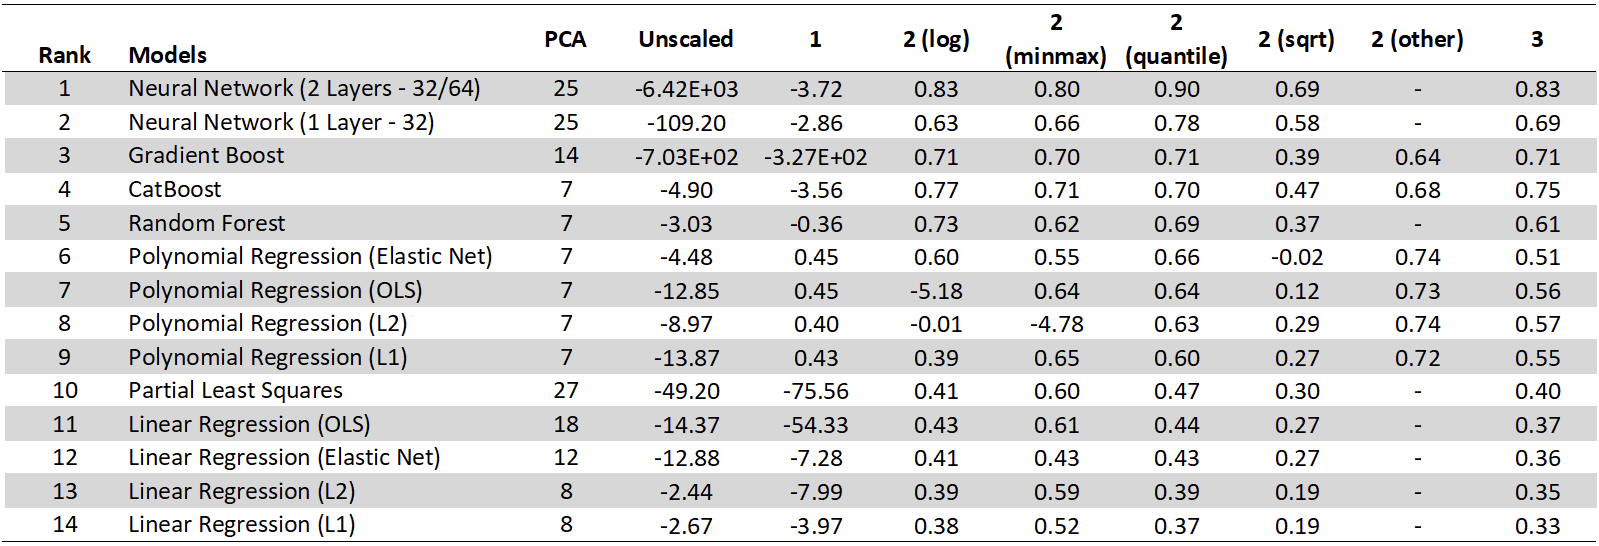
\includegraphics[width=16cm]{./media/r2results.png}
\caption{$R^{2}$ scores for each scaling method}
\end{figure}

Overall, the models that use ensemble/iterative learning processes performed the best out of the 14 models tested. The worst-performing models were the simplest, i.e. linear regression. There is a drastic improvement in results between the unscaled, method 1 scaling, and the final method of choice, 2 (log).

\subsection{Limitations of the Model}
Over the course of the project, certain limitations were identified regarding the model. The model does not consider several variables: pressure, volume, phase/state based on temperature, and the chemical environment. All of these variables will have an effect on the mole fraction in an experimental setting. The scope of the project does not encompass phase transitions or the effect of different states of matter on miscibility behaviour, hence limiting its applicability to specific conditions.\\

Another limitation lies in the use of mean mole fraction as training data for predictions, rather than exact mole fractions. Additionally, as with any ML model, there is a risk of extrapolating beyond the range of training data, potentially skewing prediction accuracy for conditions significantly different from the data set. Lastly, the effectiveness of the model is restricted to a limited range of temperatures, and extrapolation to temperatures outside this range may yield less reliable predictions. However, it must be noted that these limitations are not dead ends but rather highlight potential areas for improvement and future work.\\

\section{Future Work}
\label{section:future work}
During the preliminary investigation, a classifier was developed using a miscibility chart from Sigma-Aldrich \cite{sigma} to try to make binary predictions about compound miscibility. This model was abandoned after discovering a significant imbalance in the chart (used as training data), with only about 90 out of 1024 compound mixtures labelled as 'immiscible'. Despite this challenge, there were potential solutions to address this issue, such as oversampling the underrepresented class \cite{oversampling}. To expand on this, the binary classification model could be used to make absolute predictions for miscibility and associate them with the mole fractions of the same compound mixtures.\\

Another possible expansion of the model would be to find upper and lower critical solution temperatures, which are the temperature bounds for which a mixture is miscible\cite{ucst}. This would enable a classification prediction, and a much more useful output for a user. The ideal, and very ambitious, result of these predictions would be to allow the program to produce a temperature-composition diagram similar to the one displayed below.

\begin{figure}[ht]
\centering
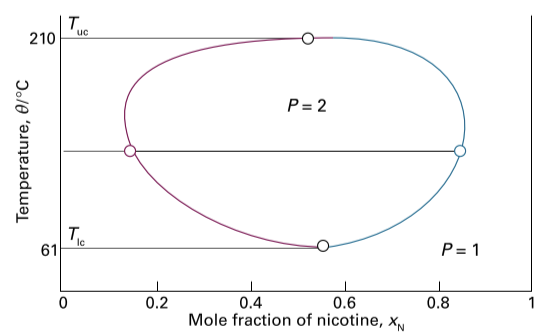
\includegraphics[width=8cm]{media/tempcomp.png}
\caption{Temperature-composition diagram for water and nicotine\cite{atkins}}
\end{figure}

\section{Conclusions}
\label{section:conclusions}
In conclusion, the model is capable of predicting the mole fractions in a binary organic compound mixture at a given temperature with an acceptable level of accuracy (90\%). Whilst testing the models, the size of the dataset was increased incrementally, with a final total of 1122 entries. After feature extraction and scaling/outlier removal, approximately 20\% of the data was lost. The final dataset was split 80:20 into a test set and validation set. However, due to time constraints, the validation set was never used in final testing.\\

The final model has barely scraped the surface of what is possible in the field of miscibility in Chemistry with machine learning, and leaves a lot of scope for further investigation in the topic.

\section{Outputs, Data \& Software Links}
All code and data is available at \url{https://github.com/joooshc/PSDI-Miscibility} \\
Plots and graphs were created using matplotlib\cite{matplotlib}
\label{section:outputs}
% INSERT OUTPUTS, DATA & SOFTWARE LINKS HERE

\bibliographystyle{vancouver}
\bibliography{References}

\end{document}